\section{\Large PROBLEM SET 1}
\subsection{PROBLEM 1}
\textit{Select some key ADCS characteristics of your mission, including orbit (e.g., LEO, MEO, GEO, HEO, Interplanetary), target attitude (e.g., Sun pointing, Inertial pointing, Earth pointing, Resident Space Object pointing), attitude state representation (e.g., Euler angles, Gibbs vector, Quaternions Direction Cosine Matrix, Euler Axis/Angle), sensors suite (Gyros, Magnetometers, Star Trackers, Earth Sensor, Sun Sensor), actuator suite (Thrusters, Magnetorquers, Reaction Wheels, Momentum Wheel, Gravity Gradient).}

The ultimate goal of the project is to work on a satellite using modern observational technologies designed to gather key environmental data on Earth. The satellite will need pointing capabilities that are controlled by the ADCS system.

\subsection{PROBLEM 2}
\textit{Conduct survey of satellites which have characteristics similar to selected project. Use internet, publications, and books as resources.}

The body axes and principal axes are \textit{co-located and aligned at the spacecraft center of mass}; on the other hand, the CAD axes is located on the bottom face of the Sun shield and its z-axis is co-linear with the aforementioned frames.

\begin{figure}[H]
\centering
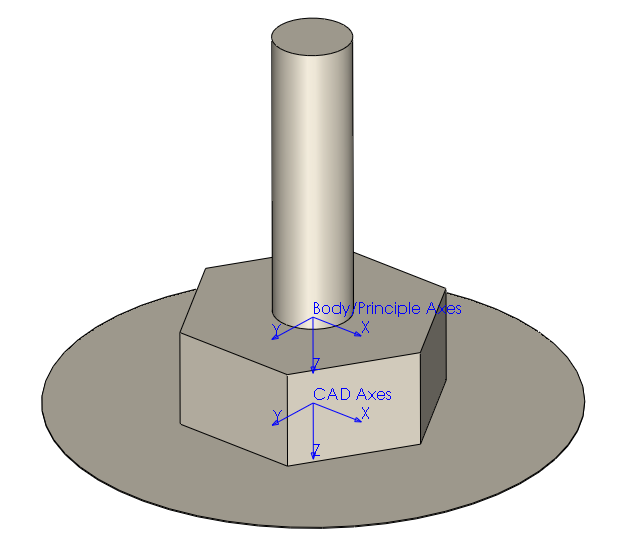
\includegraphics[scale=0.7]{Images/WMAP_CAD4.PNG}
\caption{A 3D model of the simplified satellite geometry. The body and principal axes are labeled and located at the spacecraft center of mass.}
\label{CAD model with frames}
\end{figure}


\begin{equation}
\vec{M} = \vec{I} \cdot \vec{\dot{\omega}}\ + \vec{\omega} \times \vec{I} \cdot \vec{\omega} \\ 
\end{equation}   



\begin{eqnarray}
M_x = I_{xx} \dot{\omega_x} + (I_{zz} - I_{yy})\omega_y \omega_z \nonumber \\
M_y = I_{yy} \dot{\omega_y} + (I_{xx} - I_{zz})\omega_z \omega_x \\
M_z = I_{zz} \dot{\omega_z} + (I_{yy} - I_{xx})\omega_x \omega_y \nonumber
\end{eqnarray}

\begin{equation}
I_{B} =
\begin{bmatrix} 
I_{xx} & I_{xy} & I_{xz} \\
I_{yx} & I_{yy} & I_{yz} \\ 
I_{zx} & I_{zy} & I_{zz} \\
\end{bmatrix}
=
\begin{bmatrix}
1005.5 & 0 & 0 \\
0 & 1005.5 & 0 \\ 
0 & 0 & 543.7
\end{bmatrix}
[kg/m^2].
\end{equation}

\begin{lstlisting}
function L_loc = LagrangePoints(mu)
%For a given value of mu, this function computes the location
%of all five Lagrange points for the circular restricted three
%body problem.

%Compute the location of the libration points
    l = 1 - mu;

    L_loc = zeros(5,3);

    %L1
    p_L1 = [1, 2*(mu - l), l^2 - 4*l*mu + mu^2, 2*mu*l*(l - mu) + mu - l,...
        mu^2*l^2 + 2*(l^2 + mu^2), mu^3 - l^3];
    L1roots = roots(p_L1);
    L1 = 0;
    for i = 1:5
        if (L1roots(i) > -mu) & (L1roots(i) < l)
         L1 = L1roots(i);
        end
    end
    L_loc(1,1) = L1;

    %L2
    %L3
    %L4
    %L5
end
\end{lstlisting}
